%% This is file `elsarticle-template-1-num.tex',
%%
%% Copyright 2009 Elsevier Ltd
%%
%% This file is part of the 'Elsarticle Bundle'.
%% ---------------------------------------------
%%
%% It may be distributed under the conditions of the LaTeX Project Public
%% License, either version 1.2 of this license or (at your option) any
%% later version.  The latest version of this license is in
%%    http://www.latex-project.org/lppl.txt
%% and version 1.2 or later is part of all distributions of LaTeX
%% version 1999/12/01 or later.
%%
%% Template article for Elsevier's document class `elsarticle'
%% with numbered style bibliographic references
%%
%% $Id: elsarticle-template-1-num.tex 149 2009-10-08 05:01:15Z rishi $
%% $URL: http://lenova.river-valley.com/svn/elsbst/trunk/elsarticle-template-1-num.tex $
%%
\documentclass[preprint,12pt]{elsarticle}
\usepackage[utf8]{inputenc} % указывает кодировку документа
\usepackage[T2A]{fontenc} % указывает внутреннюю кодировку TeX 
\usepackage[main=russian,english]{babel} % указывает язык документа
%% Use the option review to obtain double line spacing
%% \documentclass[preprint,review,12pt]{elsarticle}

%% Use the options 1p,twocolumn; 3p; 3p,twocolumn; 5p; or 5p,twocolumn
%% for a journal layout:
%% \documentclass[final,1p,times]{elsarticle}
%% \documentclass[final,1p,times,twocolumn]{elsarticle}
%% \documentclass[final,3p,times]{elsarticle}
%% \documentclass[final,3p,times,twocolumn]{elsarticle}
%% \documentclass[final,5p,times]{elsarticle}
%% \documentclass[final,5p,times,twocolumn]{elsarticle}

%% The graphicx package provides the includegraphics command.
\usepackage{graphicx}
%% The amssymb package provides various useful mathematical symbols
\usepackage{amssymb}
\usepackage{amsmath}
%% The amsthm package provides extended theorem environments
%% \usepackage{amsthm}

%% The lineno packages adds line numbers. Start line numbering with
%% \begin{linenumbers}, end it with \end{linenumbers}. Or switch it on
%% for the whole article with \linenumbers after \end{frontmatter}.
\usepackage{lineno}

%% natbib.sty is loaded by default. However, natbib options can be
%% provided with \biboptions{...} command. Following options are
%% valid:

%%   round  -  round parentheses are used (default)
%%   square -  square brackets are used   [option]
%%   curly  -  curly braces are used      {option}
%%   angle  -  angle brackets are used    <option>
%%   semicolon  -  multiple citations separated by semi-colon
%%   colon  - same as semicolon, an earlier confusion
%%   comma  -  separated by comma
%%   numbers-  selects numerical citations
%%   super  -  numerical citations as superscripts
%%   sort   -  sorts multiple citations according to order in ref. list
%%   sort&compress   -  like sort, but also compresses numerical citations
%%   compress - compresses without sorting
%%
%% \biboptions{comma,round}

% \biboptions{}

%% Refs
\usepackage{hyperref}
\hypersetup{
     colorlinks   = true,
     citecolor    = blue
}
\usepackage[ruled,vlined]{algorithm2e}
\usepackage{booktabs}

% Переобозначение методов Эльзивера

\makeatletter

\def\ps@pprintTitle{%
   \let\@oddhead\@empty
   \let\@evenhead\@empty
   \let\@oddfoot\@empty
   \let\@evenfoot\@oddfoot
}

\usepackage{multicol}
\usepackage{lipsum}
\usepackage{mwe}

\renewenvironment{abstract}{\global\setbox\absbox=\vbox\bgroup
  \hsize=\textwidth\def\baselinestretch{1}%
  \noindent\unskip\textbf{Abstract}
 \par\medskip\noindent\unskip\ignorespaces}
 {\egroup}

\def\keyword{%
  \def\sep{\unskip, }%
 \def\MSC{\@ifnextchar[{\@MSC}{\@MSC[2000]}}
  \def\@MSC[##1]{\par\leavevmode\hbox {\it ##1~MSC:\space}}%
  \def\PACS{\par\leavevmode\hbox {\it PACS:\space}}%
  \def\JEL{\par\leavevmode\hbox {\it JEL:\space}}%
  \global\setbox\keybox=\vbox\bgroup\hsize=\textwidth
  \normalsize\normalfont\def\baselinestretch{1}
  \parskip\z@
  \noindent\textit{Ключевые слова: Квазиньютоновские методы \sep Машинное обучение \sep Глубинное обучение \sep Глубокие нейронные сети \sep SGD \sep SGD-Momentum \sep Adam \sep LBFGS \sep Barzilai-Borwein \sep Задача оптимизации}  % <--- Edit as necessary
  \raggedright                         % Keywords are not justified.
  \ignorespaces}
%

\begin{document}

\begin{frontmatter}

%% Title, authors and addresses

\title{Стохастические квазиньютоновские методы оптимизации в контексте глубоких нейронных сетей.}

%% use the tnoteref command within \title for footnotes;
%% use the tnotetext command for the associated footnote;
%% use the fnref command within \author or \address for footnotes;
%% use the fntext command for the associated footnote;
%% use the corref command within \author for corresponding author footnotes;
%% use the cortext command for the associated footnote;
%% use the ead command for the email address,
%% and the form \ead[url] for the home page:
%%
%% \title{Title\tnoteref{label1}}
%% \tnotetext[label1]{}
%% \author{Name\corref{cor1}\fnref{label2}}
%% \ead{email address}
%% \ead[url]{home page}
%% \fntext[label2]{}
%% \cortext[cor1]{}
%% \address{Address\fnref{label3}}
%% \fntext[label3]{}


%% use optional labels to link authors explicitly to addresses:
%% \author[label1,label2]{<author name>}
%% \address[label1]{<address>}
%% \address[label2]{<address>}

\author[mipt]{А. Жогов}
\ead{zhogov.aa@phystech.edu}
\author[mipt]{М. Сысак}
\ead{sysak.ma@phystech.edu}
\author[mipt]{Б. Усеинов}
\ead{useinov.br@phystech.edu}

\address[mipt]{Московский физико-технический институт (национальный исследовательский университет), Москва, Россия}

%%\begin{abstract}
%% Text of abstract

%%\end{abstract}

\begin{keyword}
%% keywords here, in the form: keyword \sep keyword

%% MSC codes here, in the form: \MSC code \sep code
%% or \MSC[2008] code \sep code (2000 is the default)

\end{keyword}

\end{frontmatter}

%%
%% Start line numbering here if you want
%%
% \linenumbers

%% main text
\section{Введение}
\label{S:0}
В данной статье рассматриваются стохастические  квазиньютоновские методы для решения задачи классификации с помощью глубоких нейронных сетей. Квазиньютоновские методы являются широко используемыми методами в задачах выпуклой оптимизации~\cite{BBorig,BFGSorig, numopt}. При этом, для обучения нейронных сетей в качестве базового выбора алгоритма их используют редко. Это связано с тем, что в задачах глубинного обучения вычислительно затратно использовать детерминированные методы оптимизации, а стохастические версии квазиньютоновских методов обладают свойством неустойчивости~\cite{LBFGSunstable,barzilaiborwein}.

В задачах классификации, в частности, изображений, нейронные сети показывают результаты~\cite{MNISTexperiments, CIFAR10experiments}, превосходящие результаты классических методов\footnote{Такие методы как деревья решений, наивная байесовская классификация, линейная регрессия, логистичексая регрессия, градиентный бустинг и др.} машинного обучения. 
Время обучения и получаемая точность решения зависят по большей части от выбора метода оптимизации, который используется для минимизации функции потерь~\ref{eq-opt-weight}. 
В связи с этим предлагается использовать для решения задачи оптимизации стохастические модификации квазиньютоновских методов вместо стохастических методов первого порядка, традиционно применяемых к задачам обучения нейронных сетей.

% К использованию нейронных сетей, как к подходу при решении задач машинного обучения, прибегают по нескольким причинам. Во-первых, отсутствие возможности применить классические методы\footnote{Такие методы как дерево решений, наивная байесовская классификация, метод наименьших квадратов, логистичексая регрессия, градиентный бустинг и др.} в силу гетерогенности\footnote{Разнородность, инородность; наличие неодинаковых частей в структуре, в составе чего-либо. Например, наборы изображений разного размера или с разным содержанием.} набора данных. Во-вторых, требование, чтобы решение задачи отличалось высоким качеством, поскольку нейронные сети являются эффективным подходом при решении широкого спектра задач машинного обучения. Однако качество, которое показывает вышеупомянутый подход, сильно зависит от решения задачи оптимизации функции потерь (подробно об этом в разделе~\ref{S:1}). С другой стороны, квазиньютоновские методы являются очень эффективным подходом к решению задач выпуклой оптимизации, но, несмотря на это, они редко используются при решении задач, возникающих при работе с нейронными сетями. Этими причинами обусловлена идея использования стохастических модификаций квазиньютоновских методов в глубинном обучении.

Рассматриваются два стохастических квазиньютоновских метода, \linebreak один из которых является модификацией LBFGS~\cite{BFGSorig} и один~--- модификацией BB~\cite{BBorig} (подробнее о модификациях в разделах~\ref{SS:0.1}, \ref{S:2}). 
Проведено сравнение стохастических квазиньютоновских методов со стохастическими методами первого порядка~--- SGD, SGD-Momentum~\cite{GDoverview} и Adam~\cite{adam}. 
Сравнение методов проведено на задачах классификации MNIST~\cite{MNIST} с использованием полносвязной нейронной сети архитектуры~\ref{MNISTnet} и CIFAR-10~\cite{CIFAR10} с использованием сверточной нейронной сети архитектуры~\ref{CIFAR10net}.
Для сравнения методов использованы  конечное значение точности (accuracy) на отложенной выборке и время, затрачиваемое на фиксированное число итераций.

В данной работе будет проверена работоспособность стохастических квазиньютоновских методов в задачах обучения нейронных сетей. В результате методы будут отранжированы по описанным выше метрикам на каждой рассматриваемой задаче оптимизации, что позволит сделать вывод о целесообразности их использования.

\subsection{Обзор литературы}
\label{SS:0.1}
Стохастический градиентный спуск (SGD) был предложен в работе~\cite{SGDorig}.
В последующих работах были получены оценки его сходимости для выпуклых~\cite{SGDconvergence} и для невыпуклых~\cite{SGDconvergenceNonconvex} целевых функций.
Основными недостатками этого метода являются сублинейная сходимость и возможная сходимость к седловой точке, а не к локальному минимуму. Для решения этих проблем были предложены методы, описываемые ниже.

В качестве решения проблемы сублинейной скорости сходимости SGD выступал метод тяжелого шарика~\cite{Polyak}, альтернативное название которого~--- SGD-Momentum, что связано с распространенной физической интерпретацией.
Его идея состоит в добавлении дополнительного слагаемого, играющего роль инерции движения.
Доказано~\cite{HBconvergence}, что в сильно выпуклых задачах оптимизации он имеет асимптотически ту же скорость сходимости, что и градиентный спуск, но с меньшей константой.
В~\cite{GDoverview} обсуждается идея SGD-Momentum и его превосходство над SGD в задачах оптимизации, возникающих при использовании нейронных сетей в машинном обучении. 
Дальнейшей модификацией, которая обладает асимптотически более быстрой сходимостью по итерациям в задачах выпуклой оптимизации, стал ускоренный градиентный метод~\cite{NAG}, идея которого состоит в вычислении градиента в точке, смещенной относительно текущей. 
Его стохастическая модификация рассматривается в работе~\cite{NAGstochastic}.
Его достоинства по сравнению с предыдущими модификациями и обсуждение его идеи также приводятся в~\cite{GDoverview}.

Для решения проблемы сходимости к седловым точкам основным подходом является покомпонентное масштабирование градиентов. 
Первым известным подходом стал AdaGrad, предложенный в~\cite{AdaGrad}. 
Его идея состоит в масштабировании каждой компоненты градиента на корень из суммы квадратов значений этой компоненты по всем итерациям. 
Его главная проблема следует из монотонного возрастания этой суммы~--- с ростом числа итераций шаг по всем компонентам стремится к нулю. 
Эта проблема была частично решена в алгоритме RMSProp~\cite{RMSprop}, в котором сумма была заменена на скользящее экспоненциальное среднее. 
Идеи алгоритмов RMSProp и Momentum совместил в себе Adam, представленный в~\cite{adam}.

Квазиньютоновские методы чаще используются в задачах выпуклой оптимизации и на практике показывают сверхлинейную скорость сходимости~\cite{numopt}. 
В 1987 году был предложен квазиньютоновский метод BFGS~\cite{BFGSorig}, в котором на каждой итерации на основе информации о кривизне целевой функции строится плотная матрица, являющаяся оценкой обратного гессиана.
% котором на каждой итерации строится оценка обратного гессиана исходя из решения вспомогательной задачи оптимизации, требующей, чтобы новое приближение мало отличалось от предыдущего и удовлетворяло условиям, естественным для обратного гессиана (квазиньютоновскому уравнению, подробно описанному в разделах~\ref{SS:2.3} и~\ref{SS:2.4}). 
В контексте нейронных сетей недостаток этого метода состоит в неустойчивости при применении стохастической модификации напрямую, что вызвано использованием информации о кривизне различных функций на каждой итерации. Подробно эта проблема обсуждается в~\cite{LBFGSunstable}. 
Для решения этой проблемы предлагалось множество различных решений~\cite{onlineBFGS, sampledbfgs, multibatchLBFGS}, одно из которых~\cite{multibatchLBFGS} будет рассмотрено в данной работе.

Другим квазиньютоновским методом является метод \linebreak Barzilai-Borwein (BB), предложенный в~\cite{BBorig}. 
В данном методе приближение обратного гессиана строится подбором подходящего размера шага на основе информации о кривизне целевой функции.
Как и в случае с BFGS, при переходе к стохастической модификации получаемый размер шага становится неустойчивым, что показано в~\cite{barzilaiborwein}. 
Существует несколько подходов к решению этой проблемы~\cite{barzilaiborwein, BB-DL}, в данной статье будет рассмотрена одна из них~\cite{BB-DL}.

\section{Постановка задачи}
\label{S:1}
В данной работе будут рассмотрены методы, описанные в~\ref{S:2}, в контексте задачи классификации. По набору данных $\mathcal{X} = \{(\mathbf{x}_i, y_i)\}_{i=1}^n$, $\mathbf{x}_i~\in~\mathbb{R}^d$~--- вектор признаков $i$-го объекта, а $y_i \in \mathbb{Y}$~--- его метка, строится такое отображение $f\colon \, \mathbb{R}^n \rightarrow \mathbb{Y}$, чтобы наиболее точно выполнялось $\forall\, i \; f(x_i) \approx y_i$. 
Здесь $\mathbb{Y} = \{1, \dots, c\}$, где $c$~--- количество классов. 
Классический подход состоит в введении параметрического семейства функций $f\colon \, \mathbb{R}^n \times \mathbb{R}^m \rightarrow \mathbb{Y}'$, где $\mathbb{Y}' = \{\mathbf{p} \in [0, 1]^c \mid \sum_{i=1}^c p_i = 1\}$~--- пространство вероятностных распределений над $\mathbb{Y}$, а $m$~--- размерность вектора параметров. 
В рассматриваемой задаче $f$ представляет из себя глубокую нейронную сеть, а $\theta \in \mathbb{R}^m$~--- вектор ее параметров. Архитектуры сетей, рассмотренных в этой работе, описаны в разделе~\ref{S:3}.
Для подбора вектора $\theta$ вводится функция потерь $\mathcal{L}\colon \, \mathbb{Y}' \times \mathbb{Y} \rightarrow \mathbb{R}$. В данной статье используется перекрестная энтропия
\begin{equation} \label{eq-crossentropy}
    \mathcal{L}(\mathbf{p}, y) = -\log p_y
\end{equation}
Минимизация такой функции требует максимизации вероятности верного класса $p_y$, поэтому она может выступать как количественная мера качества рассматриваемой функции $f$ в контексте задачи классификации.
Оптимальное значение параметра задается как решение оптимизационной задачи
\begin{equation} \label{eq-opt-weight}
    \min_\theta F_\mathcal{X}(\theta) \triangleq \frac1n \sum_{i=1}^n \mathcal{L}(f(x_i, \theta), y_i).
\end{equation}

Рассматриваемый класс функций накладывает ограничения на применимые для решения задачи~\eqref{eq-opt-weight} методы. 
Целевая функция является дифференцируемой почти всюду, но не является выпуклой, поскольку функция $f$, задаваемая глубокой нейронной сетью, в общем случае невыпукла. 
Кроме того, часто размер выборки $n$ достаточно велик, что делает вычисление градиента $\nabla F_\mathcal{X}$ на каждой итерации численного метода вычислительно затратной задачей. 
Для ускорения градиентных методов вместо точного значения градиента используют его несмещенную оценку.
На каждой итерации случайно формируется подмножество исходной выборки $\mathcal{X}' = \{(x_{i_j}, y_{i_j})\}_{j=1}^s \subset \mathcal{X}, \, s \ll n$ (далее такие подмножества будем называть минибатчами), и градиент считается по вспомогательной функции 
\begin{equation}
    F_{\mathcal{X}'}(\theta) \triangleq \frac1s \sum_{j=1}^s \mathcal{L}(f(x_{i_j}, \theta), y_{i_j}),
\end{equation} 
то есть вместо $\nabla F_\mathcal{X}(\theta)$ используется $\nabla F_{\mathcal{X}'}(\theta)$. Как легко видеть, среднее значение функций $F_{\mathcal{X}'}$ по всем минибатчам совпадает с исходной функцией $F_\mathcal{X}$. 
Таким образом, вспомогательная функция является случайной величиной, матожидание которой равно исходной целевой функции. 
Из этого следует, что, при вычислении градиента по вспомогательной функции, градиентные методы будут в среднем вести себя так, как при вычислениях над $F_\mathcal{X}$. 
Строгое доказательство этого факта для алгоритма SGD, рассмотренного в~\ref{SS:2.1}, приведено в~\cite{SGDconvergence}.
В силу вероятностной природы методов, производящих вычисления над $F_{\mathcal{X}'}$ вместо $F_\mathcal{X}$, к их названиям принято добавлять слово <<стохастический>>. Далее в этой работе этот термин означает, что метод вычисляет градиент по $F_{\mathcal{X}'}$. 
Еще одно ограничение на применимые к задаче~\eqref{eq-opt-weight} методы вытекает из большой размерности пространства параметров $\mathbb{R}^m$, что делает невозможным применение методов второго порядка, оперирующих полным гессианом целевой функции $\nabla^2 F_\mathcal{X}(\theta)$ размерности $m \times m$. 
Эта проблема частично может быть решена применением квазиньютоновских методов, позволяющих сократить расходы по памяти и время работы по сравнению с методами второго порядка.

\section{Методы}
\label{S:2}
В этой статье будет рассмотрено два варианта стохастических модификаций квазиньютоновских методов, применяемых в глубинном обучении. Для сравнения будет использовано два стохастических градиентных метода.
% \begin{enumerate}
%     \item Стохастический градиентный спуск (SGD)~\cite{SGDconvergence}.%~--- классический метод оптимизации, используемый в решении задач машинного обучения, модификация стандартного градиентного спуска.
%     \item Adam~\cite{adam}.%~--- распространенный метод оптимизации в контексте нейронных сетей, часто используется как базовое решение при выборе алгоритма для конкретной задачи. 
%     \item SGD-BB~\cite{BB-DL}.%--- стохастическая модификация метода Barzilai-Borwein, представляющая из себя вариант выбора шага в SGD.
%     \item Multi-Batch BFGS~\cite{multibatchLBFGS}.%~--- стохастическая модификация наиболее известного квазиньютоновского метода BFGS.
%     % \item Sampled BFGS~\cite{sampledbfgs}.%~--- модификация того же метода, в которой используется другой подход к  построению приближения обратного гессиана.
% \end{enumerate}

Рассматриваемые ниже методы будут сравниваться двумя способами: на фиксированной задаче будет рассматриваться значение некоторой метрики качества (подробнее в разделе~\ref{S:3}), достигнутой за фиксированное число эпох, а также будет измеряться время, затрачиваемое на фиксированное число эпох оптимизации. 
Эпохой называют группу из числа итераций, равного отношению размера всей выборки $|\mathcal{X}|$ к размеру минибатча $|\mathcal{X}'|$. Такая группировка итераций используется для более устойчивой оценки целевой функции, в качестве которой на каждой эпохе вычисляется среднее значений $F_{\mathcal{X}'}(\theta)$ по всем итерациям этой эпохи. Такая оценка обладает меньшей дисперсией, чем каждое конкретное значение $F_{\mathcal{X}'}(\theta)$.

\subsection{Стохастический градиентный спуск (SGD)}\label{SS:2.1}
На каждой итерации генерируется минибатч $\mathcal{X}'$, после чего параметры обновляются по формуле
\begin{equation}\label{SGD}
    \theta_{k+1} = \theta_k - \eta_k \nabla F_{\mathcal{X}'} (\theta_k)
\end{equation}
Здесь последовательность длин шага $\{\eta_k\}$~--- параметр алгоритма. В данной статье используется постоянный шаг $\eta_k \equiv \eta$.
% \begin{itemize}
%     \item $\eta_k \equiv \eta$~--- фиксированный шаг. Стандартный выбор $\eta = 0.001$. В разделе~\ref{S:3} рассматривается этот подход.
%     \item Убывающая последовательность $\eta_{k+1} < \eta_k$. На практике, в задачах глубинного обучения влечет более быструю сходимость по итерациям.
%     \item <<Понижение шага на плато>>~--- стратегия выбора шага, специфичная для глубинного обучения. Примером является умножение шага на фиксированную константу $\alpha \in (0, 1)$ после фиксированного числа $r$ эпох без достаточного уменьшения значения целевой функции или метрики качества.
% \end{itemize}

Каждая итерация алгоритма требует $O(m)$ времени (без учета времени вычисления градиента), $O(m)$ памяти для хранения градиента $\nabla F_{\mathcal{X}'}(\theta)$ и $1$ вычисление градиента.

Помимо SGD в виде~\ref{SGD}, в данной работе рассматривается его модификация, называемая методом тяжелого шарика (Heavy Ball Method), или SGD-Momentum. 
На каждой итерации генерируется минибатч $\mathcal{X}'$, после чего целевая переменная обновляется по правилу
\begin{equation}\label{HB}
    \theta_{k+1} = \theta_k - \eta \nabla F_{\mathcal{X}'}(\theta_k) + \beta (\theta_k - \theta_{k+1})
\end{equation}
Анализ сходимости этого метода приведен в~\cite{HBconvergence}, где показано, что в некотором классе целевых функций он имеет меньшую константу линейной сходимости, нежели~\ref{SGD}.

Время работы и расходы по памяти этой модификации алгоритма совпадают с SGD асимптотически, но на самом деле памяти и времени требуется в два раза больше (без учета вычисления градиента), поскольку надо хранить два значения градиента вместо одного. Аналогично SGD, на каждой итерации градиент вычисляется $1$ раз.

\subsection{Adam}
В алгоритме~\ref{Adam} описан псевдокод метода Adam, представленного в~\cite{adam}. 
В этом методе на каждой итерации обновляются скользящие экспоненциальные средние, то есть величины вида
\[
    \overline{x}_{k+1} = \gamma\overline{x}_k + (1 - \gamma)x_{k+1}
\]
для коэффициента $\gamma \in (0, 1)$. 
Такие значения поддерживаются алгоритмом для градиента с коэффициентом $\beta_1$ и для покомпонентного квадрата градиента с коэффициентом $\beta_2$. 
В статье~\cite{adam} используется $\beta_1 = 0.9$ и $\beta_2 = 0.999$. 
В оригинальной статье было показано, что полученные величины являются оценками градиента и его квадрата по всей выборке, смещенными на коэффициенты $(1 - \beta_1^{t+1})$ и $(1 - \beta_2^{t+1})$ соответственно. 
Поэтому для получения несмещенных оценок следующим шагом обе величины делятся на соответствующие им коэффициенты. 
Наконец, вектор параметров обновляется на величину $-\eta \cdot m_{t+1} / (\sqrt{v_{t+1}} + \varepsilon)$. 
Поправка $\varepsilon$ здесь нужна для численной стабильности на случай близких к нулю градиентов. 
В статье~\cite{adam} используется $\varepsilon = 10^{-8}$.
От SGD такое правило отличается тем, что вместо градиента теперь используется скользящее среднее градиентов по всем итерациям, покомпонентно деленное на корень из скользящего среднего их квадратов. 
Основная мотивация состоит в том, что подобное масштабирование позволяет увеличить шаг вдоль направлений с маленьким градиентом, предотвращая сходимость к седловым точкам. Данный вопрос подробно рассматривается в~\cite{SaddlePoints} на примере алгоритма RMSprop~\cite{RMSprop}, который отличается от Adam тем, что вместо экспоненциального среднего градиентов в нем используется значение градиента на текущей итерации.

\begin{algorithm}[H]\label{Adam}
\caption {Adam\newlineЗдесь все операции с векторами покомпонентные;\newline$\beta_i^{t+1}$ обозначает возведение числа $\beta_i$ в степень $t + 1$, $i \in \{1, 2\}$.}
\SetKwInOut{Input}{Input}
\SetKwInOut{Output}{Output}
\SetAlgoLined
\Input{Число итераций $N$ \newline
        Размер шага $\eta$ \newline
        Экспоненциальные скорости затухания $\beta_1, \beta_2 \in [0, 1)$ \newline
        Начальное приближение $\theta_0$ \newline
        Поправка на численную неустойчивость $\varepsilon$}
\Output{Итоговое значение параметра $\theta_N$}
 $m_0 \leftarrow 0$\\
 $v_0 \leftarrow 0$\\
 \For{$t = 0, 1, \dotsc, N-1$}{
  Сгенерировать минибатч $\mathcal{X}_t' \subset \mathcal{X}$\\
  $g_{t+1} \leftarrow \nabla F_{\mathcal{X}_t'}(\theta_t)$\\
  $m_{t+1} \leftarrow \beta_1 \cdot m_t + (1 - \beta_1)\cdot g_{t+1}$ \\
  $v_{t+1} \leftarrow \beta_2 \cdot v_t + (1 - \beta_2)\cdot g_{t+1}^2$\\
  $\hat{m}_{t+1} \leftarrow m_{t+1} / (1 - \beta_1^{t+1})$\\
  $\hat{v}_{t+1} \leftarrow v_{t+1} / (1 - \beta_2^{t+1})$\\
  $\theta_{t+1} \leftarrow \theta_t - \eta \cdot \hat{m}_{t+1}/(\sqrt{\hat{v}_{t+1}} + \varepsilon)$
 }
 \Return{$\theta_N$}
\end{algorithm}



Данный метод имеет те же асимптотики по времени и памяти и требует такого же количества вычислений градиента, что и SGD.

\subsection{SGD-BB}\label{SS:2.3}
Главной идеей стандартного алгоритма BB является расчет размера шага с использованием информации о кривизне графика целевой функции. 
В данном методе гессиан целевой функции аппроксимируется матрицей $B_k = \eta_k^{-1}I$, где $\eta_k^{-1}$ определяется как решение квазиньютоновского уравнения
\[
    B_ks_k = y_k,
\]
которое сводится к одномерной задаче минимизации
\begin{align*}
    \min_{\eta_{t}}\| \eta_t^{-1}s_{t}-y_{t}\|_2^2,
\end{align*}
решение которой в явной форме имеет вид
$$\eta_{t} = \frac{\|s_{t}\|_2^2}{s_{t}^Ty_{t}}.$$
Здесь $s_t = \theta_{t+1} - \theta_t$ и $y_t = \nabla F_\mathcal{X}(\theta_{t+1}) - \nabla F_\mathcal{X}(\theta_t)$.

Модификация SGD-BB, представленная в~\cite{BB-DL} и псевдокод которой показан в процедуре~\ref{SGD-BB}, использует идею выделения минибатчей. Внутри эпохи $k$ фиксируется размер шага $\eta_k$, после чего совершается $T$ итераций, в течение которых вектор параметров ($k$~--- индекс эпохи, $t$~--- индекс итерации внутри эпохи) обновляется по правилу:
$$\theta_{k, 0} = \theta_{k-1, T},~\theta_{k, t+1} = \theta_{k, t} - {\eta}_k \nabla F_{\mathcal{X}_{k, t}'}(\theta_{k, t})$$
Градиент $g_{k, t}$, использующийся для нахождения ${\eta_k}$, оценивается как и в методе Adam~\ref{Adam} при помощи экспоненциального скользящего среднего
$$g_{k, t+1} = (1 - \beta) g_{k, t} + \beta \nabla F_{\mathcal{X}_{k, t}'}(\theta_{k, t})$$
В отличие от оригинального метода, разность градиентов между эпохами считается как
$$y_k = g_{k, T} - g_{k-1, T},$$
а разность векторов параметров между двумя эпохами определяется как
$$s_k = T^{-1}(\theta_{k, T} - \theta_{k-1, T}).$$
Определенные так $s_k, y_k$ дают размер шага следующей эпохи
\begin{equation}\label{eq-SGD-BB}
    \eta_{k+1} = \frac{\|s_k\|_2^2}{|s_k^Ty_k|}
\end{equation}
В отличие от оригинального BB, в знаменателе стоит модуль скалярного произведения. Это объясняется тем, что для детерминированной (то есть, не стохастической) версии алгоритма строго доказано~\cite{BBconvergence}, что $s_k^\top y_k > 0$ на каждой итерации. В стохастическом случае это не гарантируется, в том числе не гарантируется численная устойчивость \eqref{eq-SGD-BB}, для чего требуется коррекция полученного размера шага.
Значения $\eta_k$ корректируются при помощи заданных параметров $\tau_0, \tau_{\text{min}}, \tau_{\text{max}}$
$$\hat{\eta}_k = \begin{cases}
        \eta_k & \text{если } \eta_k \in \left[\frac{\tau_{\text{min}}}{k+1}, \frac {\tau_{\text{max}}}{k+1}\right], \\
        \frac{\tau_0}{k+1} & \text{иначе.}
    \end{cases}$$
\begin{algorithm}[H]\label{SGD-BB}
\caption {SGD-BB}
\SetKwInOut{Input}{Input}
\SetKwInOut{Output}{Output}
\SetAlgoLined
\Input{Число эпох $K$ \newline
        Число шагов в эпохе $T$ \newline
        Размер шага $\eta_0 = \eta_1$ \newline
        Экспоненциальная скорость затухания $\beta \in (0, 1]$ \newline
        Начальное приближение $\theta_{0, 0}$ \newline
        Корректирующие $\hat{\eta}_k$ параметры $\tau_0$, $\tau_{\text{min}}$, $\tau_{\text{max}}$
        }
\Output{
        Итоговое значение $\theta_{K, 0}$
    }
 \For{$k = 0, \ldots, K-1$}{
  \If{$k > 1$}{
    $y_{k-1} \leftarrow g_{k-1, T} - g_{k-2, T}$\\
    $s_{k-1} \leftarrow \frac{1}{T}(\theta_{k-1, T} - \theta_{k-2, T})$ \\
    $\eta_{k} \leftarrow \frac{\|s_{k-1}\|^2}{|s_{k-1}^Ty_{k-1}|}$ \\
    $\hat{\eta}_k = 
    \begin{cases}
        \eta_k & \text{если } \eta_k \in \left[\frac{\tau_{\text{min}}}{k+1}, \frac {\tau_{\text{max}}}{k+1}\right], \\
        \frac{\tau_0}{k+1} & \text{иначе.}
    \end{cases}$\\
  }
  $g_{k, 0} \leftarrow 0$ \\
 \For{$t = 0, \ldots, T-1$} {
    Сгенерировать минибатч $\mathcal{X}_{k, t}' \subset \mathcal{X}$\\ 
    $\theta_{k, t+1} \leftarrow \theta_{k, t} - \hat{\eta}_k \nabla F_{\mathcal{X}_{k, t}'}(\theta_{k, t})$ \\
    $g_{k, t+1} = (1 - \beta) g_{k, t} + \beta \nabla F_{\mathcal{X}_{k, t}'}(\theta_{k, t})$ \\
 }
 $\theta_{k+1, 0} \leftarrow \theta_{k, T}$ \\
 }
 \Return{$\theta_{K, 0}$}
\end{algorithm}

В своих экспериментах с набором данных CIFAR-10~\cite{CIFAR10} и архитектурой VGG~\cite{vgg}, авторы~\cite{BB-DL} использовали следующие значения:
\[
    T = 400, \quad \beta = 0.01, \quad \tau_0 = 0.1, \quad \tau_\text{min} = 0.1, \quad \tau_\text{max} = 10.
\]

Каждая итерация внутреннего цикла алгоритма требует $O(m)$ памяти и времени (без учета вычисления градиента) и $1$ вычисления градиента. 
Вне этого цикла на каждой эпохе происходят вычисления с теми же затратами по памяти и времени, но без вычислений градиента.

\subsection{Multi-Batch LBFGS}\label{SS:2.4}
\begin{algorithm}[H]\label{twolooprec}
\caption {two\_loop\_recursion \newline
(Вычисление произведения $H_k\mathbf{x}$ по последним $p$ парам $(y, s)$~\cite{numopt})}
\SetKwInOut{Input}{Input}
\SetKwInOut{Output}{Output}
\SetAlgoLined
\Input{Вектор $\mathbf{x}$\newline
       Набор пар $\{(y_i, s_i)\}_{i=k-p}^{k-1}$
        }
\Output{Произведение $H_k\mathbf{x}$}
 \For{$i = k-1, k-2, \dotsc, k-p$}{
  $\alpha_i \leftarrow s_i^\top \mathbf{x} / s_i^\top y_i$\\
  $\mathbf{x} \leftarrow \mathbf{x} - \alpha_i y_i$\\
 }
 $\mathbf{r} \leftarrow \dfrac{s_{k-1}^\top y_{k-1}}{y_{k-1}^\top y_{k-1}}\mathbf{x}$\\
 \For{$i = k-p, k-p+1, \dotsc, k-1$} {
    $\beta \leftarrow \dfrac{y_i^\top \mathbf{r}}{s_i^\top y_i}$\\
    $\mathbf{r} \leftarrow \mathbf{r} + s_i(\alpha_i - \beta)$\\
 }
 \Return{$\mathbf{r}$}
\end{algorithm}
Основная идея алгоритма Multi-Batch LBFGS, предложенного в~\cite{multibatchLBFGS}, состоит в построении на каждой итерации оценки обратного гессиана $H_k$ и обновлении вектора параметров по правилу
\[ 
    \theta_{k+1} = \theta_k - \eta H_k \nabla F_{\mathcal{X}_k'}(\theta_k),
\]
где $\mathcal{X}_k'$~--- минибатч. 
В отличие от BB, здесь приближение обратного гессиана $H_k$ строится таким образом, чтобы оно строго удовлетворяло квазиньютоновскому уравнению
\[s_{k+1} = H_{k+1}y_{k+1},\]
где
\[y_{k+1} = \nabla F_{\mathcal{X}_{k+1}' \cap \mathcal{X}_k'}(\theta_{k+1}) - \nabla F_{\mathcal{X}_{k+1}' \cap \mathcal{X}_k'}(\theta_k) \quad s_{k+1} = \theta_{k+1} - \theta_k\]
В дальнейшем будем обозначать $O_k = \mathcal{X}_{k+1}' \cap \mathcal{X}_k'$. 
Такие условия накладывают ограничение на процедуру генерации батчей: требуется, чтобы два батча на соседних итерациях имели пересечение фиксированного размера $|O_k| = l < s = |\mathcal{X}_k'|$. 
Это требование обусловлено тем, что на практике при вычислении градиентов для $y_{k+1}$ по разным подмножествам выборки $\mathcal{X}$ оценка обратного гессиана $H_k$ становится неустойчивой~\cite{LBFGSunstable}. 
Multi-Batch LBFGS хранит последние $p$ пар $(y_i, s_i)$, и по ним вычисляет произведение $H_k \nabla F_{\mathcal{X}_k'}(\theta_k)$ с помощью процедуры two\_loop\_recursion, вынесенной в алгоритм~\ref{twolooprec} и описанной в~\cite{numopt}. 
После каждой итерации пара $(y_{k - p}, s_{k - p})$ заменяется на новую пару $(y_k, s_k)$. 
Псевдокод всего метода приведен в алгоритме~\ref{MB-LBFGS}.\\
\begin{algorithm}[H]\label{MB-LBFGS}
\caption {Multi-Batch LBFGS}
\SetKwInOut{Input}{Input}
\SetKwInOut{Output}{Output}
\SetAlgoLined
\Input{Число итераций $N$ \newline
Начальное приближение $\theta_0$ \newline
Размер памяти $p$ \newline
Размер пересечения минибатчей $l$ \newline
Размер шага $\eta$}
\Output{Итоговое значение параметра $\theta_N$}
 Сгенерировать минибатч $\mathcal{X}_0'$\\
 $C \leftarrow \varnothing$\\
 \For{$k = 0, 1, \dotsc, N-1$}{
  $g_k \leftarrow \nabla F_{\mathcal{X}_k'}(\theta_k)$\\
  $p_k \leftarrow \text{two\_loop\_recursion}(g_k, C)$\\
  $\theta_{k+1} \leftarrow \theta_k - \eta \cdot p_k$\\
  Создать минибатч $\mathcal{X}_{k+1}'$\\
  $O_k \leftarrow \mathcal{X}_{k+1}' \cap \mathcal{X}_k'$\\
  $s_{k+1} \leftarrow \theta_{k+1} - \theta_k$\\
  $y_{k+1} \leftarrow \nabla F_{O_k}(\theta_{k+1}) - \nabla F_{O_k}(\theta_k)$\\
  \eIf{$k \ge p$}{
   $C \leftarrow C \cup \{(y_{k+1}, s_{k+1})\} \setminus \{(y_{k+1-p}, s_{k+1-p})\}$
  }{
   $C \leftarrow C \cup \{(y_{k+1}, s_{k+1})\}$
  }
 }
\end{algorithm}
В статье~\cite{multibatchLBFGS} утверждается, что $p$ целесообразно выбирать из отрезка $[2, 20]$, отношение размера пересечения минибатчей к размеру одного минибатча $l/s$ может быть любым числом из интервала $(0, 0.5)$, выбор авторов оригинальной статьи~--- $0.25$. 
% Стандартный размер шага $\eta = 1$, что мотивировано наличием матрицы $H_k$, которая представляет из себя альтернативу умножению градиента на скаляр и сама по себе играет роль <<длины шага>>.

Каждая итерация алгоритма требует $O(mp)$ времени (без учета вычисления градиента) и памяти, а также трех вычислений градиента.

% \subsection{Sampled LBFGS}
% \begin{algorithm}[H]\label{sampleCurvature}
% \caption {C\_generate (Генерация случайных пар $(y, s)$)}
% \SetKwInOut{Input}{Input}
% \SetKwInOut{Output}{Output}
% \SetAlgoLined
% \Input{Начальное приближение $\theta_0$ \newline
% Минибатч $\mathcal{X}'$ \newline
% Размер памяти $p$ \newline
% Радиус отбора $\rho$}
% \Output{Множество пар $C$\newline
%         Градиент в начальной точке $\nabla F_{\mathcal{X}'}(\theta_0)$}
%  $g \leftarrow \nabla F_{\mathcal{X}'}(\theta_0)$\\
%  $C \leftarrow \varnothing$\\
%  \For{$i = 1, 2, \dotsc, p$}{
%   Сгенерировать случайный $\sigma \in \mathbb{R}^m$, $\|\sigma\|_2 = 1$\\
%   $\theta \leftarrow \theta_0 + \rho\cdot\sigma$\\
%   $s \leftarrow \theta_0 - \theta$\\
%   $y \leftarrow  g - \nabla F_{\mathcal{X}'}(\theta)$\\
%   $C \leftarrow C \cup \{(y, s)\}$
%  }
%  \Return{$C$, $g$}
% \end{algorithm}
% Данный метод, предложенный в \cite{sampledbfgs}, является альтернативой методу LBFGS. 
% Его отличие от алгоритма~\ref{MB-LBFGS} в том, что, вместо истории пар $(y_i, s_i)$ по последним $p$ итерациям, на каждой итерации генерируется набор из $p$ случайных пар $C = \{(y_i, s_i)\}_{i=1}^p$ с помощью процедуры~\ref{sampleCurvature}. 
% Это позволяет снять ограничение на пересечение последовательных минибатчей, но при этом увеличивает количество операций за одну итерацию алгоритма. 
% Пары $(y_i, s_i)$ задают информацию о кривизне графика целевой функции, поэтому их вычисление в малой окрестности текущей точки позволяет получить приемлемую с практической точки зрения локальную оценку обратного гессиана и избежать проблем с устойчивостью, которые были упомянуты в предыдущем разделе. 
% Алгоритм вычисления приближения обратного гессиана $H_k$ совпадает с таковым для предыдущего метода и описан в процедуре~\ref{twolooprec}. Псевдокод метода Sampled LBFGS приведен в~\ref{sampledLBFGS}.

% \begin{algorithm}[H]\label{sampledLBFGS}
% \caption {Sampled LBFGS}
% \SetKwInOut{Input}{Input}
% \SetKwInOut{Output}{Output}
% \SetAlgoLined
% \Input{Число итераций $N$ \newline
% Начальное приближение $\theta_0$ \newline
% Размер памяти $p$ \newline
% Радиус отбора $\rho$ \newline
% Размер шага $\eta$}
% \Output{Итоговое значение параметра $\theta_N$}
%  \For{$k = 0, 1, \dotsc, N-1$}{
%   Сгенерировать минибатч $\mathcal{X}_k'$\\
%   $C, g_k \leftarrow \text{C\_generate}(\theta_k, \mathcal{X}_k', p, \rho)$\\
%   $p_k \leftarrow \text{two\_loop\_recursion}(g_k, C)$\\
%   $\theta_{k+1} \leftarrow \theta_k - \eta \cdot p_k$\\
%  }
% \end{algorithm}

% % Стандартные значения для $p$ и $\eta$ совпадают с соответствующими значениями для предыдущего метода.
% Для радиуса отбора авторы статьи~\cite{sampledbfgs} использовали значение $\rho = 1$.
% Размер памяти в оригинальной статье был принят равным $p = 10$. 

% Асимптотики по времени и памяти данного метода совпадают с Multi-Batch LBFGS. 
% При этом за итерацию градиент вычисляется $p+1$ раз, что при $p \gg 3$ требует больше времени за итерацию, чем в случае Multi-Batch модификации~\ref{MB-LBFGS}, которая требует трех вычислений.

\section{Эксперименты}
\label{S:3}
В данном разделе будут рассмотрены два примера применения методов оптимизации, описанных в разделе~\ref{S:2}, к задаче классификации, описанной в разделе~\ref{S:1}. В каждом эксперименте для конкретной задачи строится и обучается нейронная сеть подходящей архитектуры. В качестве метрики качества обученной модели используется доля правильных ответов на отложенной выборке $\mathcal{X}_\text{test}$, с данными из которой модель не взаимодействовала во время обучения. Эту величину будем обозначать $\mathcal{A}_s$ (от слова accuracy), где $s$~--- число эпох обучения.
\subsection{MNIST}\label{SS:3.1}
В этом эксперименте метод SGD-BB сравнивается с SGD-momentum и Adam на примере оптимизации полносвязной нейронной сети~\ref{MNISTnet} на наборе данных MNIST \cite{MNIST}. Задача состоит в определении цифры на изображении~(Рис.\ref{mnist-example}) размера $28 \times 28$.
\begin{table}[h!]
\caption{Архитектура нейронной сети в эксперименте с MNIST}
\centering
\begin{tabular}{{p{0.15\textwidth}|p{0.8\textwidth}}}
\toprule
№ & Слой \\
\midrule
0:~вход & $28\times28$ изображение, преобразованное в вектор размерности $784$ \\
1: & Полносвязный, $128$ нейронов, входных связей $784$, с активацией ReLU \\
2: & Полносвязный, $64$ нейрона, входных связей $128$, с активацией ReLU \\
3:~выход & Полносвязный, $10$ нейронов, входных связей $64$, с активацией LogSoftMax \\
\bottomrule
\end{tabular}
\label{MNISTnet}
\end{table}
\begin{figure*}[ht!]
\centering

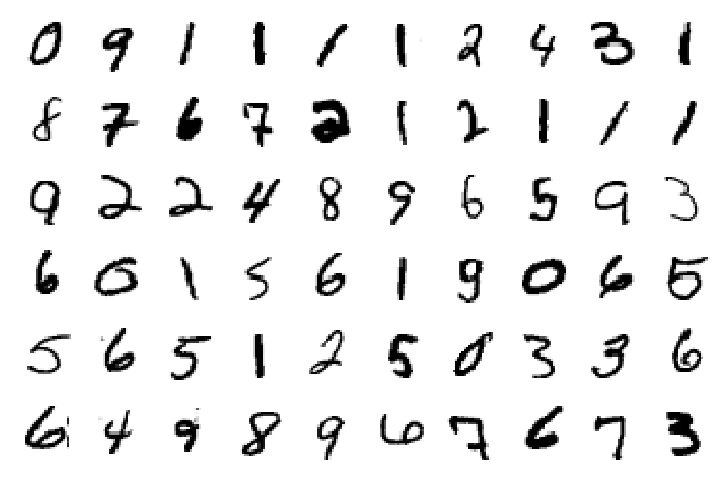
\includegraphics[height=.45\textwidth]{mnist_example.pdf}
\caption{Примеры изображений в эксперименте с MNIST}
\label{mnist-example}
\end{figure*}
\begin{table}[h!]
\caption{Результаты 15 эпох обучения нейронной сети в эксперименте с MNIST}
\centering
\begin{tabular}{{p{0.3\textwidth}|p{0.2\textwidth}p{0.1\textwidth}p{0.1\textwidth}p{0.1\textwidth}}}
\toprule
Метод &  Время, 15 эпох &  $\mathcal{A}_5$ &  $\mathcal{A}_{10}$ &  $\mathcal{A}_{15}$ \\
\midrule
               SGD & \textbf{2.81 мин} & 89.72 & 91.46 & 92.69 \\
 SGD-momentum & 3.10 мин & 95.81 & \textbf{97.19} & 97.30 \\
              Adam & 3.80 мин & \textbf{96.89} & 97.17 & \textbf{97.57} \\
                SGD-BB & 3.33 мин & 91.57 & 95.11 & 97.01 \\
\bottomrule
\end{tabular}
\end{table}
\begin{figure*}[ht!]
    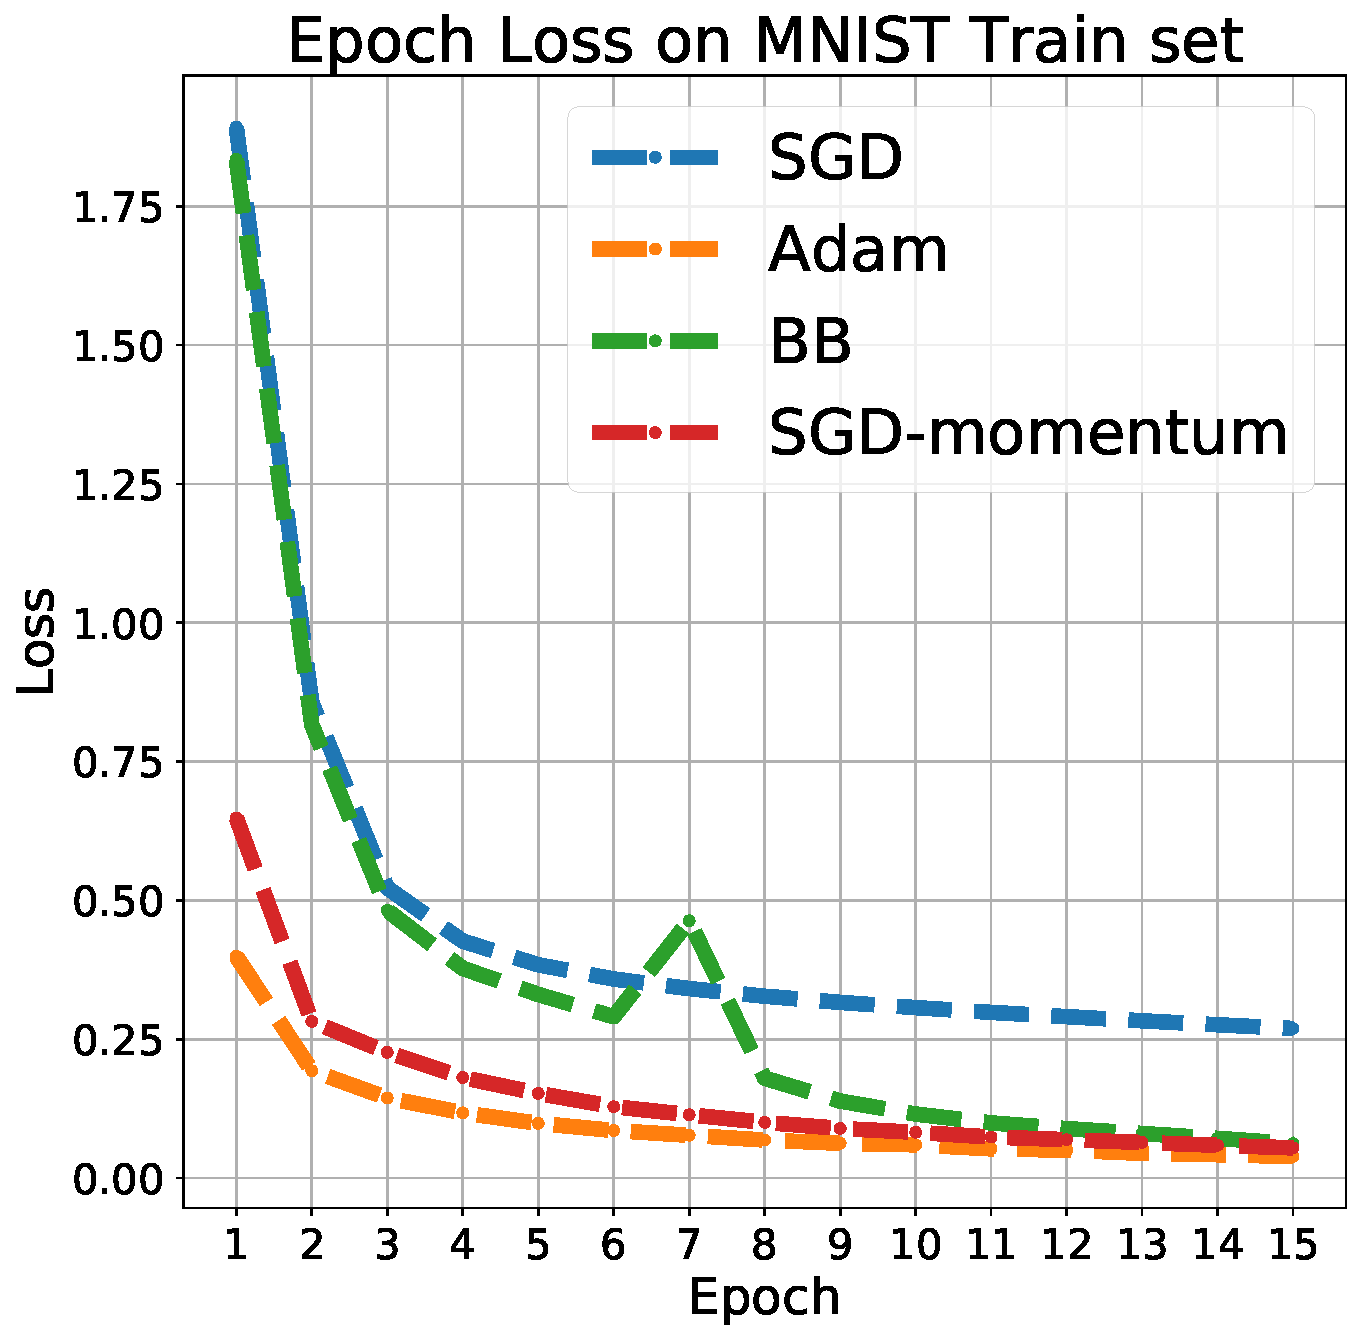
\includegraphics[height=.33\textwidth]{mnist_train_losses.pdf}\hfill
    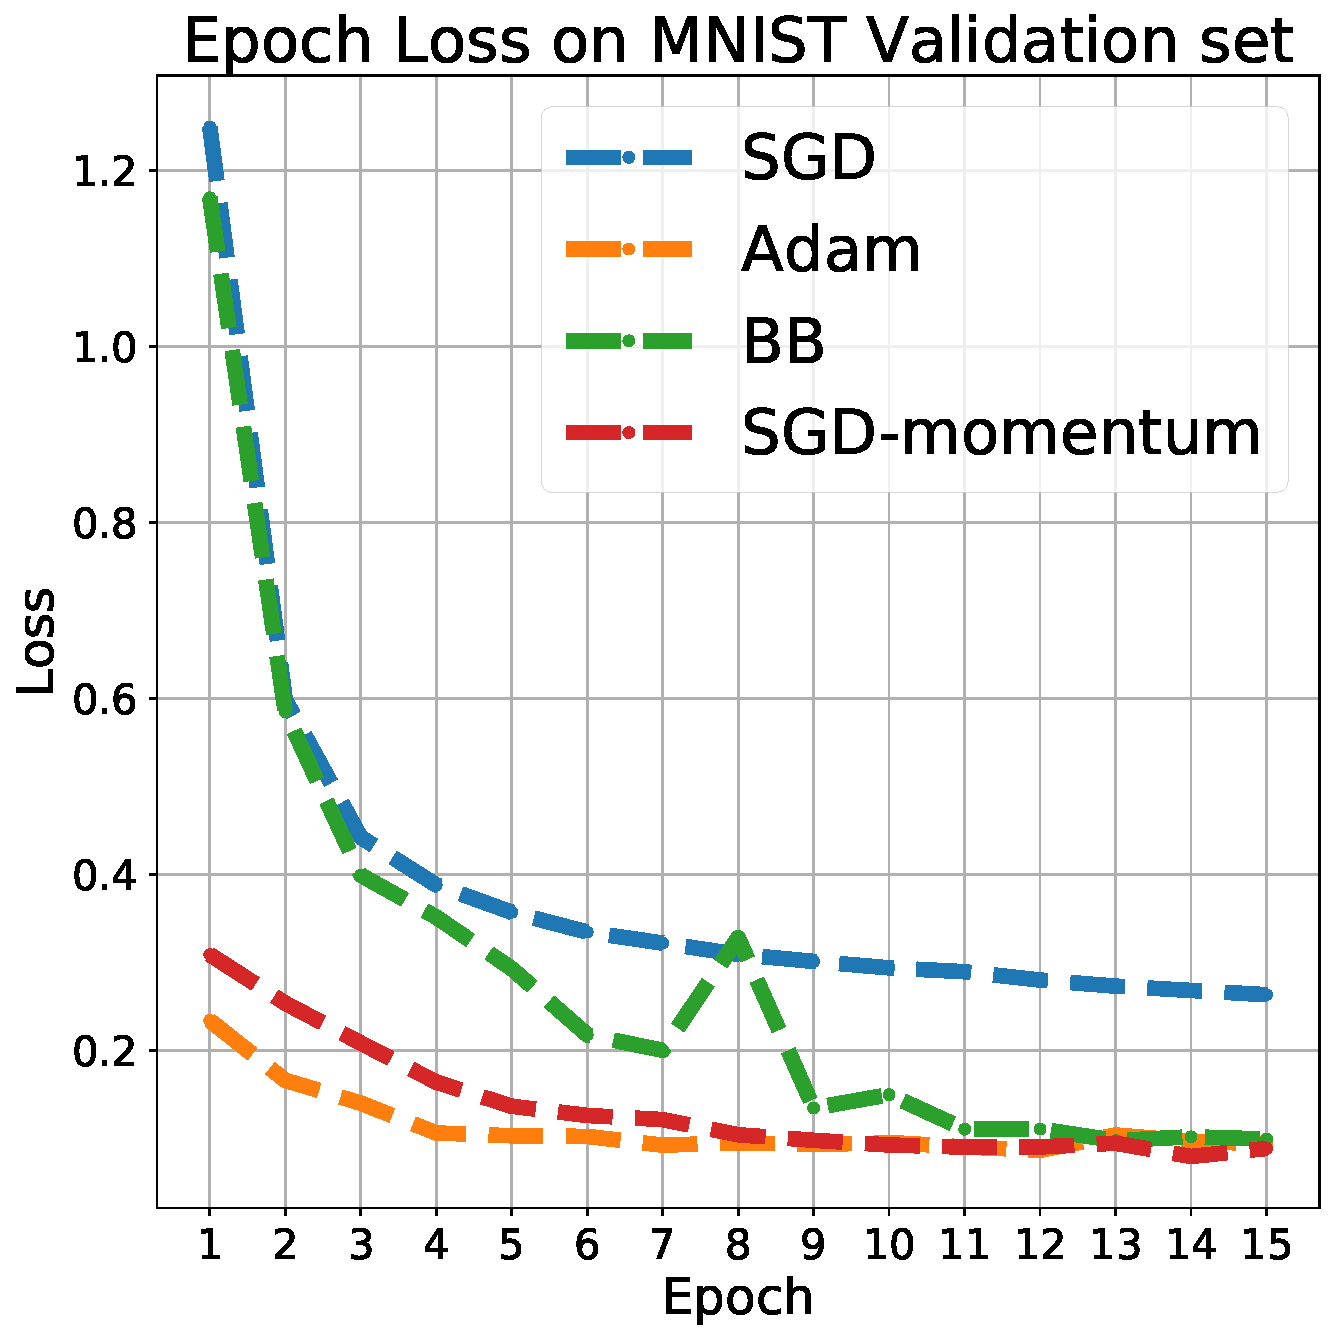
\includegraphics[height=.33\textwidth]{mnist_val_losses.pdf}\hfill
    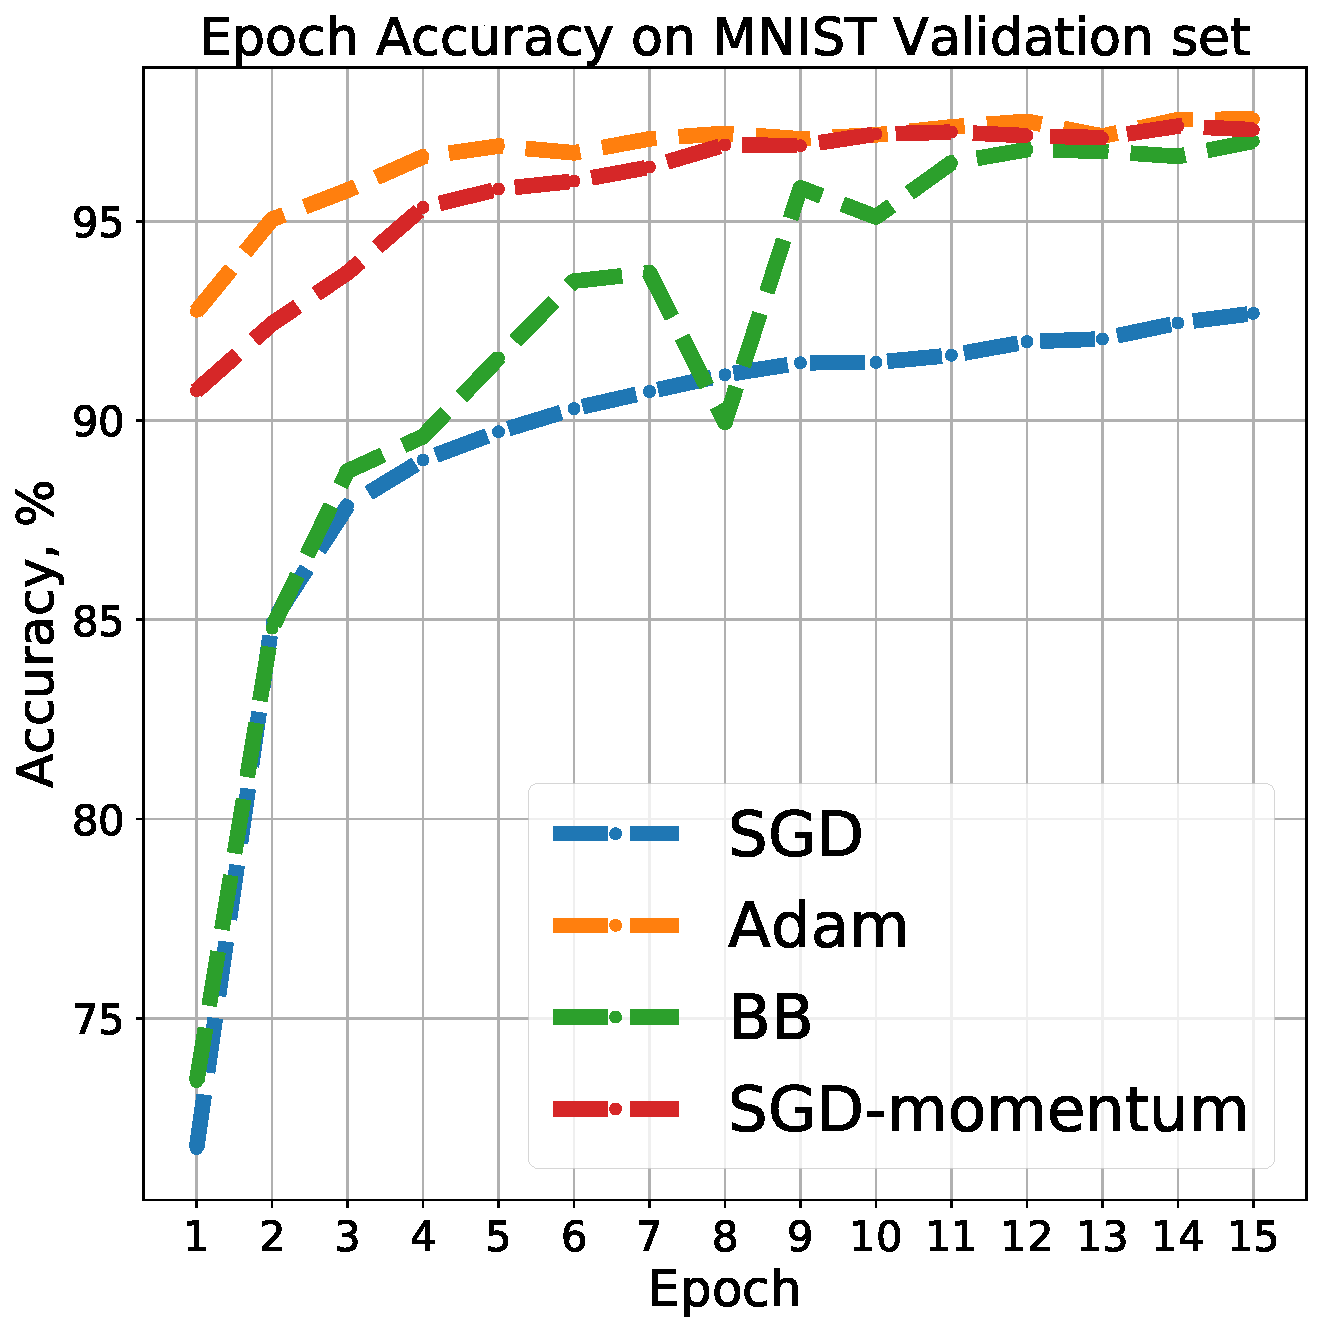
\includegraphics[height=.33\textwidth]{mnist_val_accuracy.pdf}
\caption{Графики сходимости методов в эксперименте с MNIST}
\end{figure*}

По времени все четыре алгоритма практически идентичны. 
Adam работает немного дольше, поскольку он делает больше вычислений на каждой итерации. 
По достигаемой метрике качества Adam и SGD-Momentum показывают близкие к идентичным результаты, превосходя два других алгоритма на первых итерациях. 
На последних эпохах SGD-BB достигает сравнимого с ними качества. 
SGD-BB оказывается более точным, чем SGD, что показывает эффективность процедуры выбора шага, описанной в алгоритме~\ref{SGD-BB}.
Полученные результаты согласуются с результатами, приведенными в статье~\cite{BB-DL}.

\subsection{CIFAR-10}
В этом эксперименте MultiBatch LBFGS и SGD-BB сравниваются с Adam и SGD при оптимизации сверточной нейронной сети~\ref{CIFAR10net} на данных CIFAR-10~\cite{CIFAR10}. 
Этот набор данных состоит из изображений~(Рис.\ref{cifar-example}) размера $32 \times 32$, которые необходимо классифицировать на $10$ классов.
\begin{table}[h!]
\caption{Архитектура нейронной сети в эксперименте с CIFAR-10}
\centering
\begin{tabular}{{p{0.15\textwidth}|p{0.8\textwidth}}}
\toprule
№ & Слой \\
\midrule
0:~вход & \text{$32\times32$ изображение} \\
1: & Сверточный, $6\ 5\times5$ ядер (шаг=1), с активацией ReLU \\
2: & Субдискретизирующий по максимуму, окно $2\times2$ (шаг=2)\\
3: & Сверточный, $16\ 5\times5$ ядер (шаг=1), с активацией ReLU\\
4: & Полносвязный, $1000$ нейронов, с активацией ReLU \\
5:~выход & Полносвязный, $10$ нейронов \\
\bottomrule
\end{tabular}
\label{CIFAR10net}
\end{table}
\begin{figure*}[ht!]

\centering
    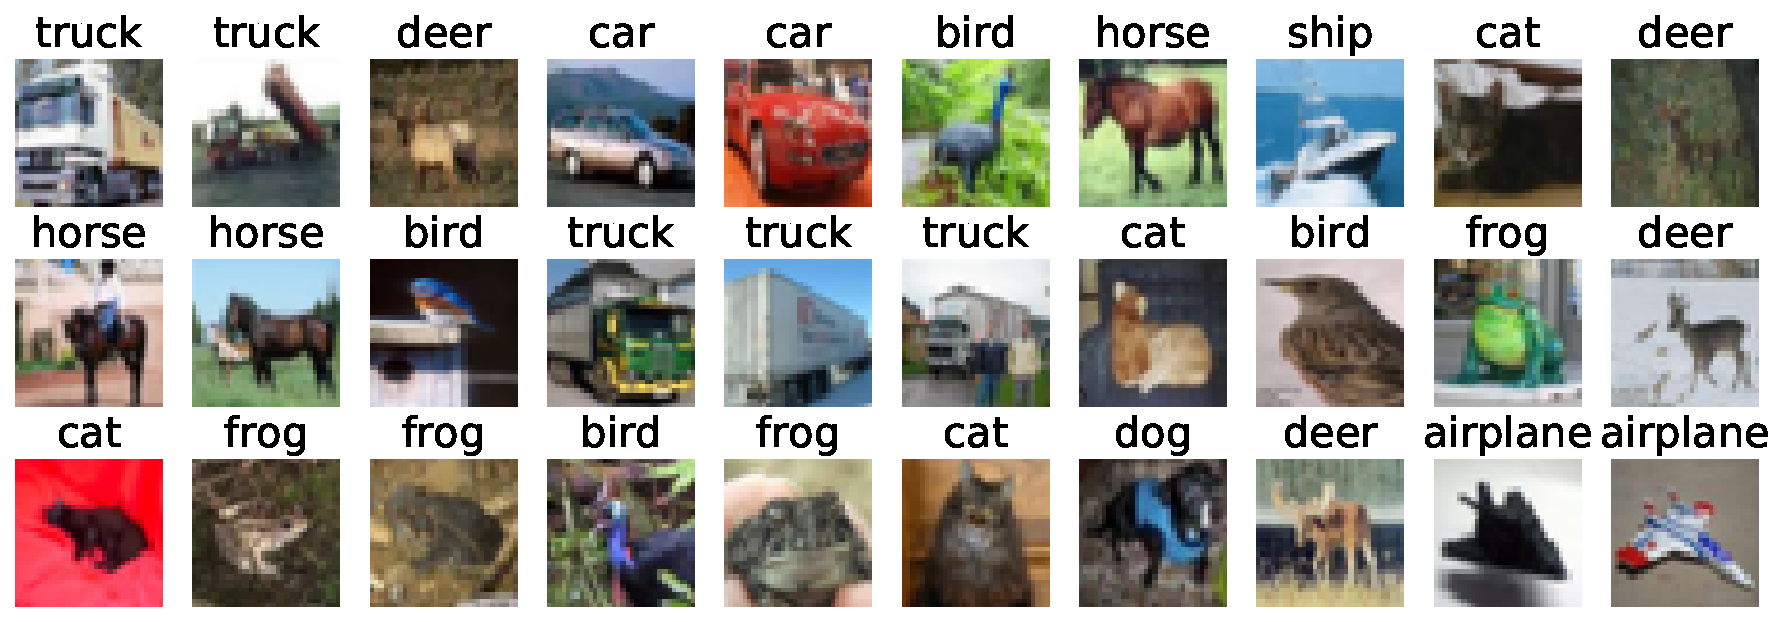
\includegraphics[height=.33\textwidth]{cifar_example.pdf}
\caption{Примеры изображений в эксперименте с CIFAR-10}
\label{cifar-example}
\end{figure*}
\begin{table}[h!]
\caption{Результаты 15 эпох обучения нейронной сети в эксперименте с CIFAR-10}
\centering
\begin{tabular}{{p{0.3\textwidth}|p{0.2\textwidth}p{0.1\textwidth}p{0.1\textwidth}p{0.1\textwidth}}}
\toprule
Метод &  Время, 15 эпох &  $\mathcal{A}_5$ &  $\mathcal{A}_{10}$ &  $\mathcal{A}_{15}$ \\
\midrule
             LBFGS &  6.37 мин &  42.39 &   44.85 &   47.32 \\
              Adam &  5.35 мин &  \textbf{52.07} &   \textbf{59.98} &   \textbf{62.38} \\
               SGD &  5.19 мин &  10.06 &   15.79 &   24.26 \\
 SGD-momentum &  5.40 мин &  39.43 &   47.70 &   51.11 \\
                SGD-BB &  \textbf{5.16 мин} &  28.98 &   47.48 &   54.68 \\
\bottomrule
\end{tabular}
\end{table}
\begin{figure*}[ht!]
    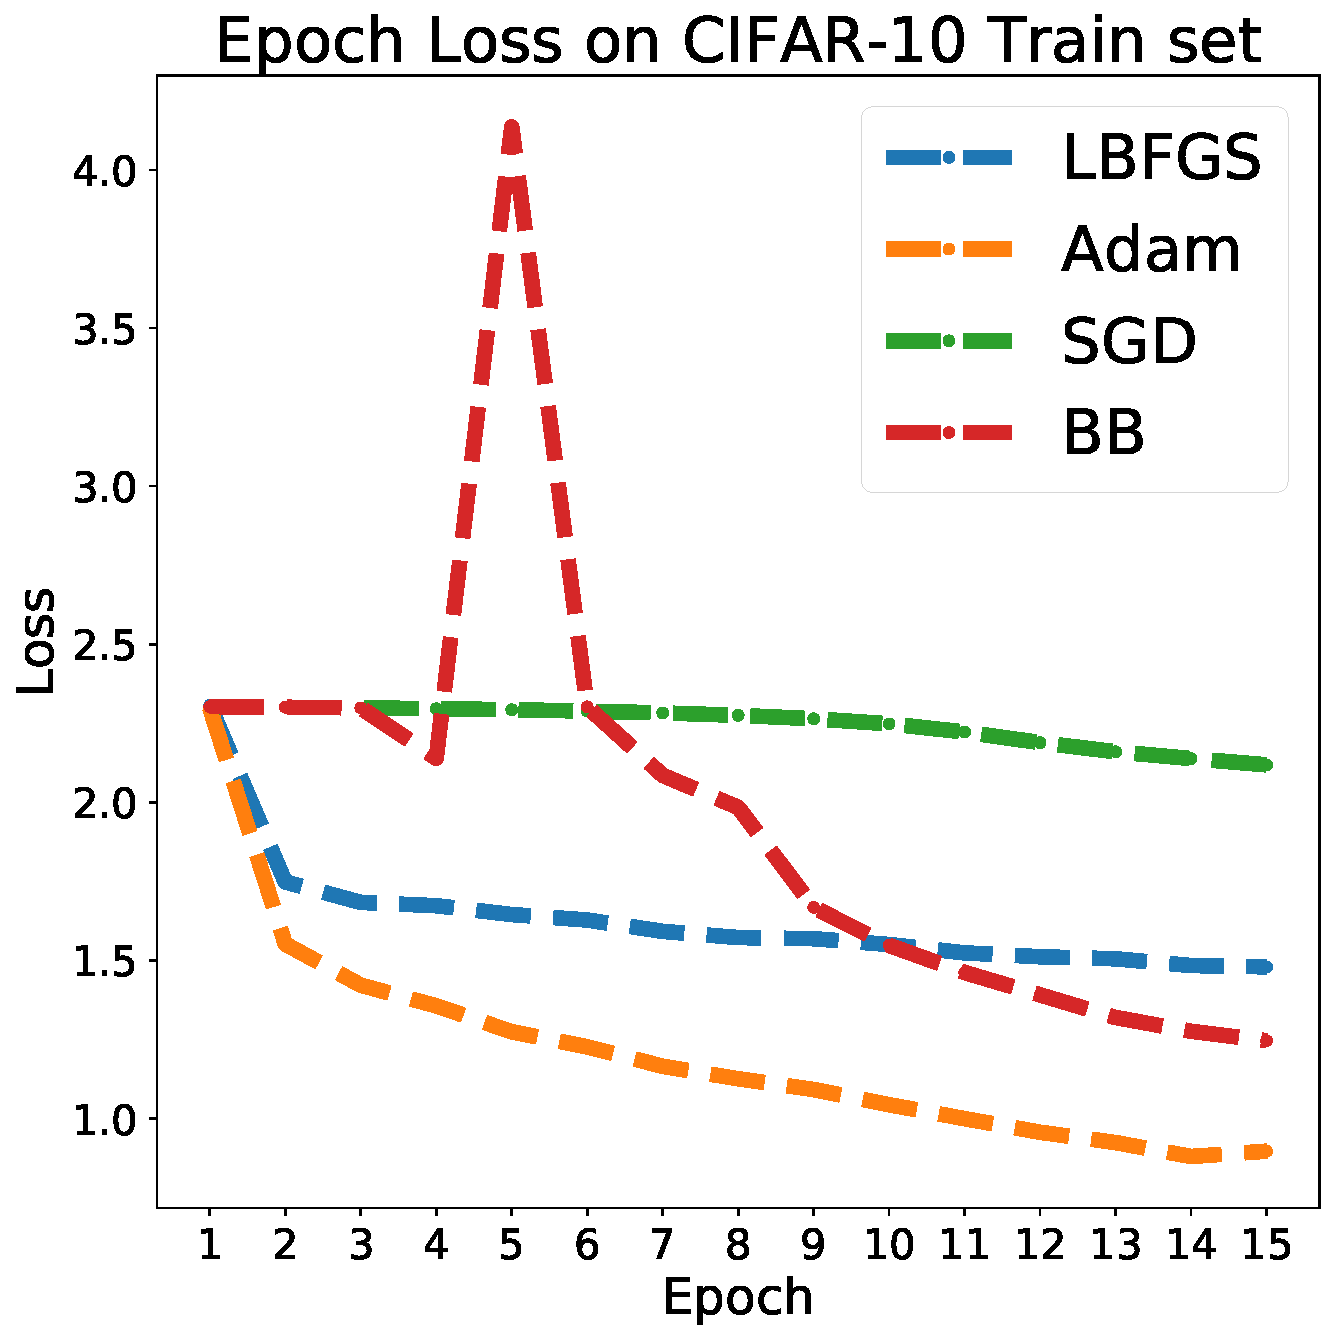
\includegraphics[height=.33\textwidth]{cifar_train_losses.pdf}\hfill
    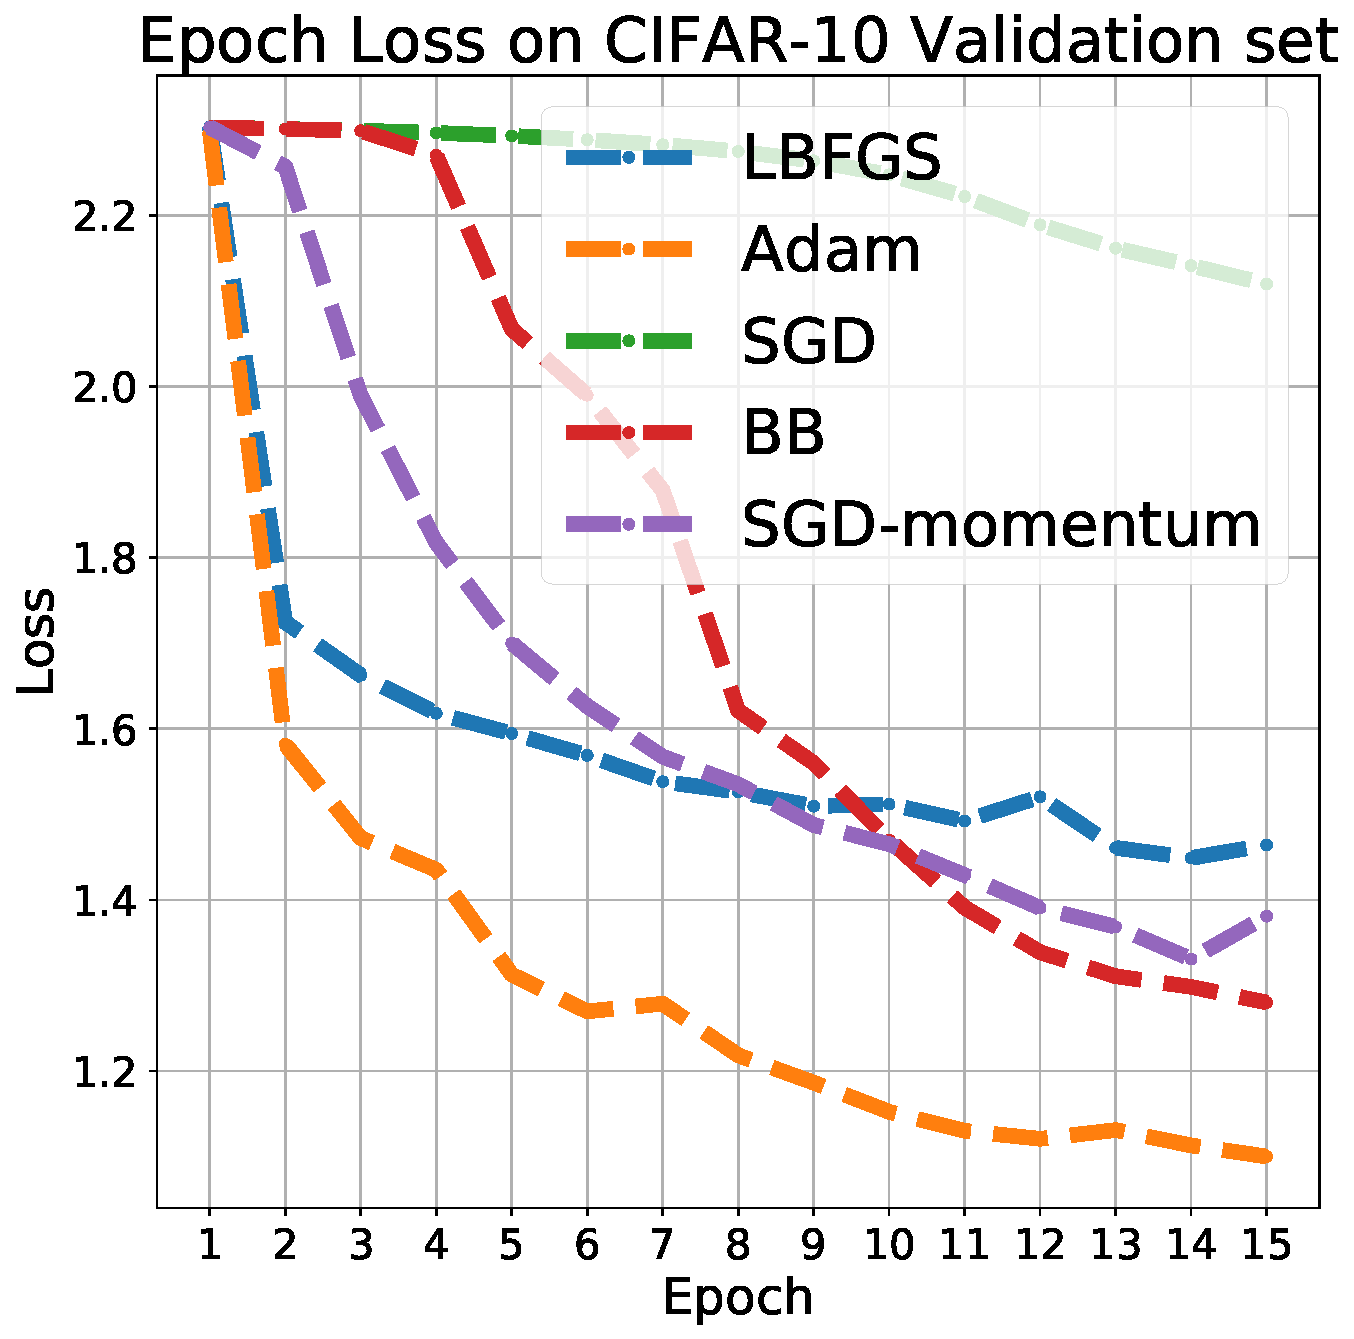
\includegraphics[height=.33\textwidth]{cifar_val_losses.pdf}\hfill
    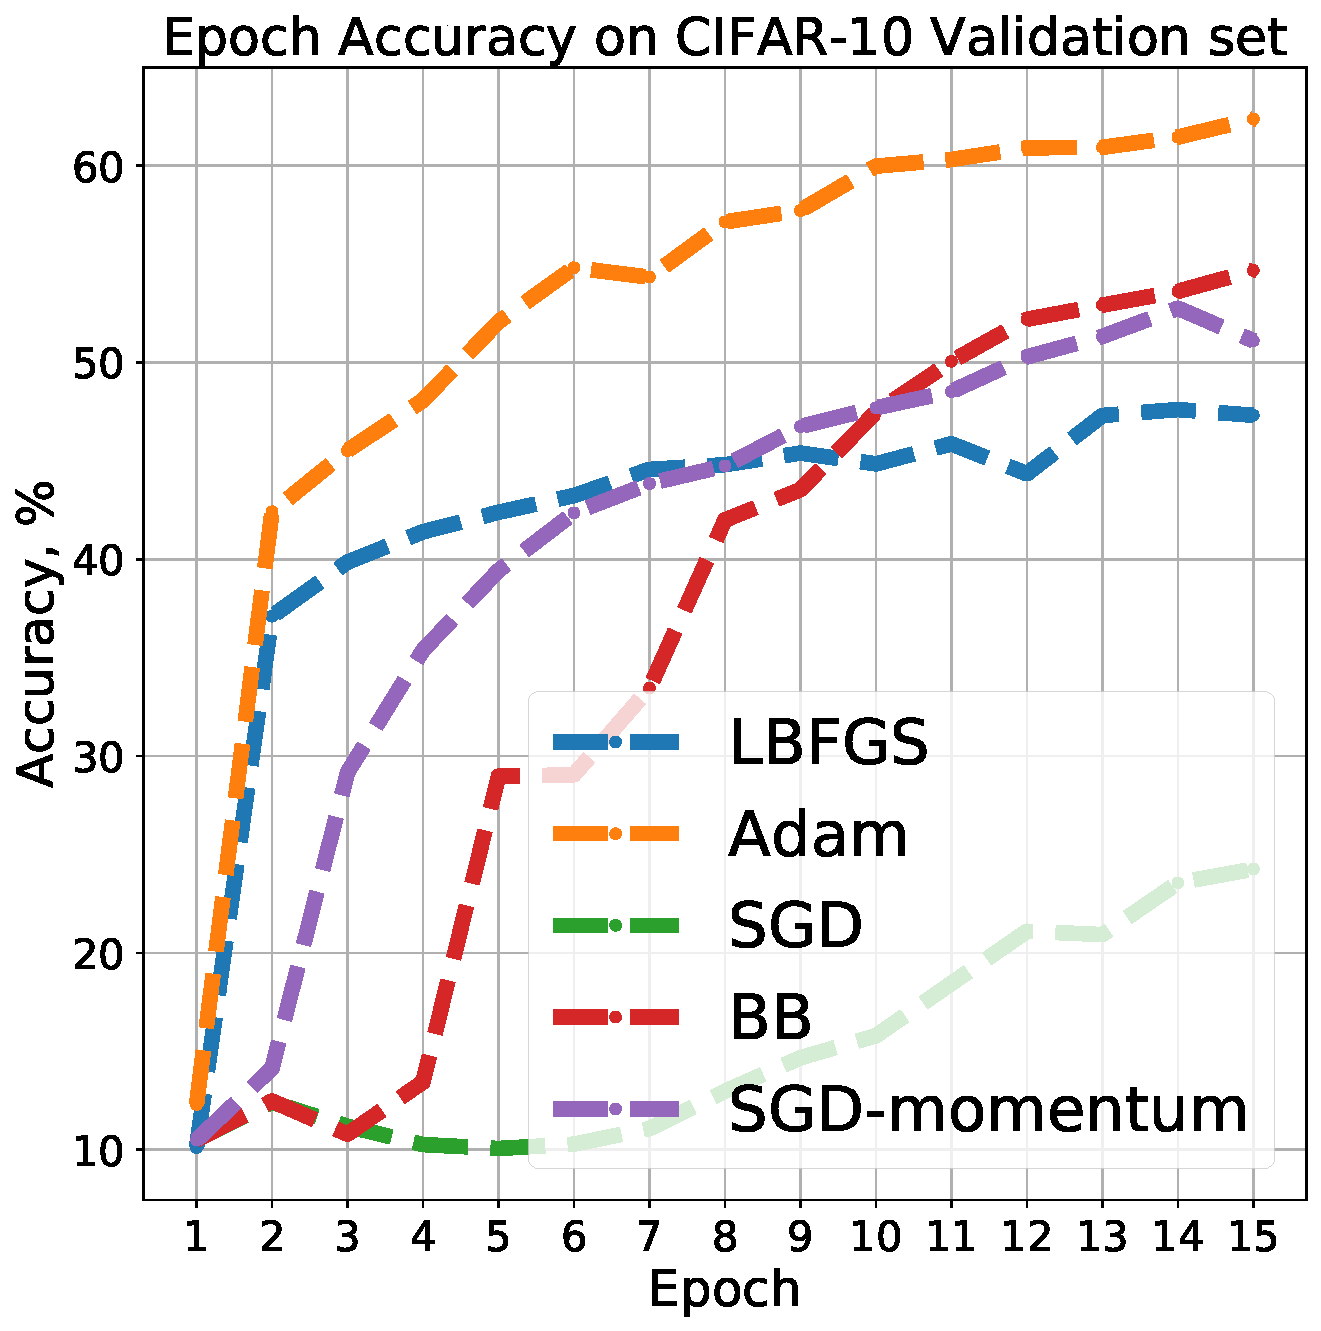
\includegraphics[height=.33\textwidth]{cifar_val_accuracy.pdf}
\caption{Графики сходимости методов в эксперименте с CIFAR-10}
\end{figure*}

Как и в эксперименте~\ref{SS:3.1}, алгоритмы Adam, SGD, SGD-Momentum и SGD-BB практически не отличаются по затрачиваемому времени, в то время как MB-LBFGS работает дольше на четверть. 
Это объясняется тем, что этот метод требует нескольких вычислений градиента на каждой итерации. 
По достигаемой точности SGD показывает результат хуже остальных алгоритмов, что является распространенным явлением при использовании постоянного шага в глубоких нейронных сетях. 
Adam показывает лучший результат в данном эксперименте.
SGD-BB, SGD-Momentum и MB-LBFGS показывают схожие между собой результаты. Первый оказывается предпочтительнее остальных в силу большего значения метрики качества при меньшем времени работы.
В оригинальной статье~\cite{multibatchLBFGS} MB-LBFGS сравнивается с SGD, результаты, полученные ее авторами, согласуются с результатами этого раздела.

\section{Заключение}
\label{S:4}
В результате экспериментов получена предпочтительность квазиньютоновских методов алгоритму SGD, так как последний сходится за большее число итераций, как на практике и происходит в задачах выпуклой оптимизации. Полученные результаты согласуются с результатами экспериментов, приведенных в~\cite{multibatchLBFGS, BB-DL}.
Квазиньютоновские методы показывают результаты, сопоставимые по качеству с результатами методов Adam и SGD-Momentum.
% По сравнению с методом Adam, прослеживаются сопоставимые по качеству результаты у квазиньютоновских методов в терминах сходимости по итерациям.
% В терминах времени фиксированного числа итераций получено, что все рассматриваемые методы сравнимы, за исключением модификаций LBFGS, выполняющих больше вычислений на каждой итерации.
За исключением LBFGS, который работает на $20\%$ дольше остальных методов, все рассматриваемые методы сравнимы по затрачиваемому на фиксированное число итераций времени.

В данной работе без рассмотрения остались стохастические модификации квазиньютоновского метода DFP~\cite{DFPorig}, который, однако, на практике используется меньше, чем BFGS~\cite{numopt}. % 139 страница
Кроме того, остается открытым вопрос о применимости стохастической модификации метода Ньютона~\cite{numopt}, время работы которого необходимо сравнить со временем, затрачиваемым квазиньютоновскими методами, для получения вывода о практической предпочтительности использования приближения гессиана. 
Задачей оптимизации, оставшейся без рассмотрения, является обучение рекуррентной нейронной сети в задаче классификации текста.
К ее решению могут быть применены все описанные выше методы оптимизации.

%% The Appendices part is started with the command \appendix;
%% appendix sections are then done as normal sections
%% \appendix

%% \section{}
%% \label{}

%% References
%%
%% Following citation commands can be used in the body text:
%% Usage of \cite is as follows:
%%   \cite{key}          ==>>  [#]
%%   \cite[chap. 2]{key} ==>>  [#, chap. 2]
%%   \citet{key}         ==>>  Author [#]

%% References with bibTeX database:

% \bibliographystyle{model1-num-names}

%% New version of the num-names style
\bibliographystyle{elsarticle-num-names}
\bibliography{bibliography.bib}

%% Authors are advised to submit their bibtex database files. They are
%% requested to list a bibtex style file in the manuscript if they do
%% not want to use model1-num-names.bst.

%% References without bibTeX database:

% \begin{thebibliography}{00}

%% \bibitem must have the following form:
%%   \bibitem{key}...
%%

% \bibitem{}

% \end{thebibliography}


\end{document}

%%
%% End of file `elsarticle-template-1-num.tex'.